% Options for packages loaded elsewhere
\PassOptionsToPackage{unicode}{hyperref}
\PassOptionsToPackage{hyphens}{url}
\PassOptionsToPackage{dvipsnames,svgnames,x11names}{xcolor}
%
\documentclass[
  11pt,
]{article}

\usepackage{amsmath,amssymb}
\usepackage{iftex}
\ifPDFTeX
  \usepackage[T1]{fontenc}
  \usepackage[utf8]{inputenc}
  \usepackage{textcomp} % provide euro and other symbols
\else % if luatex or xetex
  \usepackage{unicode-math}
  \defaultfontfeatures{Scale=MatchLowercase}
  \defaultfontfeatures[\rmfamily]{Ligatures=TeX,Scale=1}
\fi
\usepackage{lmodern}
\ifPDFTeX\else  
    % xetex/luatex font selection
\fi
% Use upquote if available, for straight quotes in verbatim environments
\IfFileExists{upquote.sty}{\usepackage{upquote}}{}
\IfFileExists{microtype.sty}{% use microtype if available
  \usepackage[]{microtype}
  \UseMicrotypeSet[protrusion]{basicmath} % disable protrusion for tt fonts
}{}
\makeatletter
\@ifundefined{KOMAClassName}{% if non-KOMA class
  \IfFileExists{parskip.sty}{%
    \usepackage{parskip}
  }{% else
    \setlength{\parindent}{0pt}
    \setlength{\parskip}{6pt plus 2pt minus 1pt}}
}{% if KOMA class
  \KOMAoptions{parskip=half}}
\makeatother
\usepackage{xcolor}
\usepackage[margin=1in]{geometry}
\setlength{\emergencystretch}{3em} % prevent overfull lines
\setcounter{secnumdepth}{5}
% Make \paragraph and \subparagraph free-standing
\makeatletter
\ifx\paragraph\undefined\else
  \let\oldparagraph\paragraph
  \renewcommand{\paragraph}{
    \@ifstar
      \xxxParagraphStar
      \xxxParagraphNoStar
  }
  \newcommand{\xxxParagraphStar}[1]{\oldparagraph*{#1}\mbox{}}
  \newcommand{\xxxParagraphNoStar}[1]{\oldparagraph{#1}\mbox{}}
\fi
\ifx\subparagraph\undefined\else
  \let\oldsubparagraph\subparagraph
  \renewcommand{\subparagraph}{
    \@ifstar
      \xxxSubParagraphStar
      \xxxSubParagraphNoStar
  }
  \newcommand{\xxxSubParagraphStar}[1]{\oldsubparagraph*{#1}\mbox{}}
  \newcommand{\xxxSubParagraphNoStar}[1]{\oldsubparagraph{#1}\mbox{}}
\fi
\makeatother

\usepackage{color}
\usepackage{fancyvrb}
\newcommand{\VerbBar}{|}
\newcommand{\VERB}{\Verb[commandchars=\\\{\}]}
\DefineVerbatimEnvironment{Highlighting}{Verbatim}{commandchars=\\\{\}}
% Add ',fontsize=\small' for more characters per line
\usepackage{framed}
\definecolor{shadecolor}{RGB}{241,243,245}
\newenvironment{Shaded}{\begin{snugshade}}{\end{snugshade}}
\newcommand{\AlertTok}[1]{\textcolor[rgb]{0.68,0.00,0.00}{#1}}
\newcommand{\AnnotationTok}[1]{\textcolor[rgb]{0.37,0.37,0.37}{#1}}
\newcommand{\AttributeTok}[1]{\textcolor[rgb]{0.40,0.45,0.13}{#1}}
\newcommand{\BaseNTok}[1]{\textcolor[rgb]{0.68,0.00,0.00}{#1}}
\newcommand{\BuiltInTok}[1]{\textcolor[rgb]{0.00,0.23,0.31}{#1}}
\newcommand{\CharTok}[1]{\textcolor[rgb]{0.13,0.47,0.30}{#1}}
\newcommand{\CommentTok}[1]{\textcolor[rgb]{0.37,0.37,0.37}{#1}}
\newcommand{\CommentVarTok}[1]{\textcolor[rgb]{0.37,0.37,0.37}{\textit{#1}}}
\newcommand{\ConstantTok}[1]{\textcolor[rgb]{0.56,0.35,0.01}{#1}}
\newcommand{\ControlFlowTok}[1]{\textcolor[rgb]{0.00,0.23,0.31}{\textbf{#1}}}
\newcommand{\DataTypeTok}[1]{\textcolor[rgb]{0.68,0.00,0.00}{#1}}
\newcommand{\DecValTok}[1]{\textcolor[rgb]{0.68,0.00,0.00}{#1}}
\newcommand{\DocumentationTok}[1]{\textcolor[rgb]{0.37,0.37,0.37}{\textit{#1}}}
\newcommand{\ErrorTok}[1]{\textcolor[rgb]{0.68,0.00,0.00}{#1}}
\newcommand{\ExtensionTok}[1]{\textcolor[rgb]{0.00,0.23,0.31}{#1}}
\newcommand{\FloatTok}[1]{\textcolor[rgb]{0.68,0.00,0.00}{#1}}
\newcommand{\FunctionTok}[1]{\textcolor[rgb]{0.28,0.35,0.67}{#1}}
\newcommand{\ImportTok}[1]{\textcolor[rgb]{0.00,0.46,0.62}{#1}}
\newcommand{\InformationTok}[1]{\textcolor[rgb]{0.37,0.37,0.37}{#1}}
\newcommand{\KeywordTok}[1]{\textcolor[rgb]{0.00,0.23,0.31}{\textbf{#1}}}
\newcommand{\NormalTok}[1]{\textcolor[rgb]{0.00,0.23,0.31}{#1}}
\newcommand{\OperatorTok}[1]{\textcolor[rgb]{0.37,0.37,0.37}{#1}}
\newcommand{\OtherTok}[1]{\textcolor[rgb]{0.00,0.23,0.31}{#1}}
\newcommand{\PreprocessorTok}[1]{\textcolor[rgb]{0.68,0.00,0.00}{#1}}
\newcommand{\RegionMarkerTok}[1]{\textcolor[rgb]{0.00,0.23,0.31}{#1}}
\newcommand{\SpecialCharTok}[1]{\textcolor[rgb]{0.37,0.37,0.37}{#1}}
\newcommand{\SpecialStringTok}[1]{\textcolor[rgb]{0.13,0.47,0.30}{#1}}
\newcommand{\StringTok}[1]{\textcolor[rgb]{0.13,0.47,0.30}{#1}}
\newcommand{\VariableTok}[1]{\textcolor[rgb]{0.07,0.07,0.07}{#1}}
\newcommand{\VerbatimStringTok}[1]{\textcolor[rgb]{0.13,0.47,0.30}{#1}}
\newcommand{\WarningTok}[1]{\textcolor[rgb]{0.37,0.37,0.37}{\textit{#1}}}

\providecommand{\tightlist}{%
  \setlength{\itemsep}{0pt}\setlength{\parskip}{0pt}}\usepackage{longtable,booktabs,array}
\usepackage{calc} % for calculating minipage widths
% Correct order of tables after \paragraph or \subparagraph
\usepackage{etoolbox}
\makeatletter
\patchcmd\longtable{\par}{\if@noskipsec\mbox{}\fi\par}{}{}
\makeatother
% Allow footnotes in longtable head/foot
\IfFileExists{footnotehyper.sty}{\usepackage{footnotehyper}}{\usepackage{footnote}}
\makesavenoteenv{longtable}
\usepackage{graphicx}
\makeatletter
\newsavebox\pandoc@box
\newcommand*\pandocbounded[1]{% scales image to fit in text height/width
  \sbox\pandoc@box{#1}%
  \Gscale@div\@tempa{\textheight}{\dimexpr\ht\pandoc@box+\dp\pandoc@box\relax}%
  \Gscale@div\@tempb{\linewidth}{\wd\pandoc@box}%
  \ifdim\@tempb\p@<\@tempa\p@\let\@tempa\@tempb\fi% select the smaller of both
  \ifdim\@tempa\p@<\p@\scalebox{\@tempa}{\usebox\pandoc@box}%
  \else\usebox{\pandoc@box}%
  \fi%
}
% Set default figure placement to htbp
\def\fps@figure{htbp}
\makeatother
% definitions for citeproc citations
\NewDocumentCommand\citeproctext{}{}
\NewDocumentCommand\citeproc{mm}{%
  \begingroup\def\citeproctext{#2}\cite{#1}\endgroup}
\makeatletter
 % allow citations to break across lines
 \let\@cite@ofmt\@firstofone
 % avoid brackets around text for \cite:
 \def\@biblabel#1{}
 \def\@cite#1#2{{#1\if@tempswa , #2\fi}}
\makeatother
\newlength{\cslhangindent}
\setlength{\cslhangindent}{1.5em}
\newlength{\csllabelwidth}
\setlength{\csllabelwidth}{3em}
\newenvironment{CSLReferences}[2] % #1 hanging-indent, #2 entry-spacing
 {\begin{list}{}{%
  \setlength{\itemindent}{0pt}
  \setlength{\leftmargin}{0pt}
  \setlength{\parsep}{0pt}
  % turn on hanging indent if param 1 is 1
  \ifodd #1
   \setlength{\leftmargin}{\cslhangindent}
   \setlength{\itemindent}{-1\cslhangindent}
  \fi
  % set entry spacing
  \setlength{\itemsep}{#2\baselineskip}}}
 {\end{list}}
\usepackage{calc}
\newcommand{\CSLBlock}[1]{\hfill\break\parbox[t]{\linewidth}{\strut\ignorespaces#1\strut}}
\newcommand{\CSLLeftMargin}[1]{\parbox[t]{\csllabelwidth}{\strut#1\strut}}
\newcommand{\CSLRightInline}[1]{\parbox[t]{\linewidth - \csllabelwidth}{\strut#1\strut}}
\newcommand{\CSLIndent}[1]{\hspace{\cslhangindent}#1}

\usepackage{booktabs}
\usepackage{longtable}
\usepackage{array}
\usepackage{multirow}
\usepackage{wrapfig}
\usepackage{float}
\usepackage{colortbl}
\usepackage{pdflscape}
\usepackage{tabu}
\usepackage{threeparttable}
\usepackage{threeparttablex}
\usepackage[normalem]{ulem}
\usepackage{makecell}
\usepackage{xcolor}
\makeatletter
\@ifpackageloaded{caption}{}{\usepackage{caption}}
\AtBeginDocument{%
\ifdefined\contentsname
  \renewcommand*\contentsname{Table of contents}
\else
  \newcommand\contentsname{Table of contents}
\fi
\ifdefined\listfigurename
  \renewcommand*\listfigurename{List of Figures}
\else
  \newcommand\listfigurename{List of Figures}
\fi
\ifdefined\listtablename
  \renewcommand*\listtablename{List of Tables}
\else
  \newcommand\listtablename{List of Tables}
\fi
\ifdefined\figurename
  \renewcommand*\figurename{Figure}
\else
  \newcommand\figurename{Figure}
\fi
\ifdefined\tablename
  \renewcommand*\tablename{Table}
\else
  \newcommand\tablename{Table}
\fi
}
\@ifpackageloaded{float}{}{\usepackage{float}}
\floatstyle{ruled}
\@ifundefined{c@chapter}{\newfloat{codelisting}{h}{lop}}{\newfloat{codelisting}{h}{lop}[chapter]}
\floatname{codelisting}{Listing}
\newcommand*\listoflistings{\listof{codelisting}{List of Listings}}
\makeatother
\makeatletter
\makeatother
\makeatletter
\@ifpackageloaded{caption}{}{\usepackage{caption}}
\@ifpackageloaded{subcaption}{}{\usepackage{subcaption}}
\makeatother

\usepackage{bookmark}

\IfFileExists{xurl.sty}{\usepackage{xurl}}{} % add URL line breaks if available
\urlstyle{same} % disable monospaced font for URLs
\hypersetup{
  pdftitle={Human-like Decision Making in Agent-Based Models: A Comparative Study of Large Language Model Agents versus Traditional Utility Maximization in the Schelling Segregation Model},
  pdfauthor={Andreas Pape, Carl Lipo, etc.},
  pdfkeywords={agent-based modeling, large language
models, segregation, Schelling model, artificial intelligence, complex
systems},
  colorlinks=true,
  linkcolor={blue},
  filecolor={Maroon},
  citecolor={Blue},
  urlcolor={Blue},
  pdfcreator={LaTeX via pandoc}}


\title{Human-like Decision Making in Agent-Based Models: A Comparative
Study of Large Language Model Agents versus Traditional Utility
Maximization in the Schelling Segregation Model}
\author{Andreas Pape, Carl Lipo, etc.}
\date{2025-06-14}

\begin{document}
\maketitle
\begin{abstract}
We present a novel approach to agent-based modeling by replacing
traditional utility-maximizing agents with Large Language Model (LLM)
agents that make human-like residential decisions. Using the classic
Schelling segregation model as our testbed, we compare three agent
types: (1) traditional mechanical agents using best-response dynamics,
(2) LLM agents making decisions based on current neighborhood context,
and (3) LLM agents with persistent memory of past interactions and
relationships. Our results reveal that LLM agents converge to stable
residential patterns 2.2× faster than mechanical agents while achieving
similar final segregation levels (\textasciitilde55\% vs 58\%
like-neighbors). Notably, memory-enhanced LLM agents demonstrate the
fastest convergence (84 steps vs 187 for mechanical agents) and a 53.8\%
reduction in extreme segregation (``ghetto'' formation). These findings
suggest that incorporating human-like decision-making through LLMs can
produce more realistic dynamics in agent-based models of social
phenomena, with important implications for urban planning and policy
analysis.
\end{abstract}


\section{Introduction}\label{introduction}

The Schelling segregation model (Schelling 1971) has been a cornerstone
of agent-based modeling (ABM) for over five decades, demonstrating how
mild individual preferences for similar neighbors can lead to stark
residential segregation. Traditional implementations use
utility-maximizing agents that relocate when the proportion of like
neighbors falls below a threshold. While mathematically elegant, this
approach may not capture the complexity of human residential
decision-making, which involves social relationships, personal history,
and contextual factors beyond simple utility calculations.

Recent advances in Large Language Models (LLMs) offer an unprecedented
opportunity to incorporate more realistic human-like decision-making
into agent-based models. LLMs trained on vast corpora of human text can
simulate nuanced responses to complex social situations, potentially
bridging the gap between simplified mathematical models and real-world
behavior (Park et al. 2023; Argyle et al. 2023).

In this paper, we present a comparative study of three agent types
within the Schelling framework:

\begin{enumerate}
\def\labelenumi{\arabic{enumi}.}
\tightlist
\item
  \textbf{Mechanical agents}: Traditional utility-maximizing agents
  using best-response dynamics
\item
  \textbf{Standard LLM agents}: Agents whose decisions are generated by
  LLMs based on current neighborhood context
\item
  \textbf{Memory LLM agents}: LLM agents with persistent memory of past
  interactions and relationships
\end{enumerate}

Our key research questions are: - How do convergence dynamics differ
between mechanical and LLM-based agents? - Do LLM agents produce
different segregation patterns than traditional agents? - What is the
impact of memory on residential stability and segregation outcomes?

\section{Methods}\label{methods}

\subsection{Experimental Design}\label{experimental-design}

We implemented a comparative framework using identical environmental
conditions across all agent types. The simulation environment consists
of a 15×15 grid (225 cells) populated with 50 agents equally divided
between two types (25 Type A ``red'' and 25 Type B ``blue''), yielding a
density of 22.2\%.

\subsection{Agent Implementations}\label{agent-implementations}

\subsubsection{Mechanical Baseline}\label{mechanical-baseline}

Traditional agents use a utility function based on the proportion of
like neighbors: \[U_i = \begin{cases} 
1 & \text{if } p_i \geq \tau \\
0 & \text{otherwise}
\end{cases}\] where \(p_i\) is the proportion of like neighbors and
\(\tau = 0.5\) is the satisfaction threshold.

\subsubsection{LLM Agents}\label{llm-agents}

LLM agents receive contextual prompts describing their current
neighborhood and make decisions based on the generated response. For
Standard LLM agents:

\begin{verbatim}
You are a [Type A/B] resident. Your current neighborhood has:
- X Type A neighbors
- Y Type B neighbors  
- Z empty houses nearby
Would you prefer to stay or move? If move, which empty house?
\end{verbatim}

Memory LLM agents receive additional context about their residential
history and past interactions.

\subsection{Metrics}\label{metrics}

We evaluate segregation using five complementary metrics: -
\textbf{Share}: Average proportion of like neighbors -
\textbf{Clusters}: Number of contiguous same-type regions -
\textbf{Distance}: Average distance between different-type agents -
\textbf{Ghetto rate}: Number of agents in homogeneous neighborhoods -
\textbf{Mix deviation}: Deviation from perfect integration

\subsection{Statistical Analysis}\label{statistical-analysis}

All experiments were run with 2 replicates for each condition. We use
Mann-Whitney U tests for pairwise comparisons and report effect sizes
using Cohen's d.

\section{Results}\label{results}

\subsection{Convergence Dynamics}\label{convergence-dynamics}

\begin{Shaded}
\begin{Highlighting}[]
\CommentTok{\# Prepare convergence data}
\NormalTok{conv\_summary }\OtherTok{\textless{}{-}}\NormalTok{ convergence\_data }\SpecialCharTok{\%\textgreater{}\%}
  \FunctionTok{mutate}\NormalTok{(}
    \AttributeTok{agent\_type =} \FunctionTok{case\_when}\NormalTok{(}
\NormalTok{      experiment }\SpecialCharTok{==} \StringTok{"mechanical\_baseline"} \SpecialCharTok{\textasciitilde{}} \StringTok{"Mechanical Baseline"}\NormalTok{,}
\NormalTok{      experiment }\SpecialCharTok{==} \StringTok{"standard\_llm"} \SpecialCharTok{\textasciitilde{}} \StringTok{"Standard LLM"}\NormalTok{,}
\NormalTok{      experiment }\SpecialCharTok{==} \StringTok{"memory\_llm"} \SpecialCharTok{\textasciitilde{}} \StringTok{"Memory LLM"}
\NormalTok{    )}
\NormalTok{  )}

\CommentTok{\# A. Convergence time distribution}
\NormalTok{p1 }\OtherTok{\textless{}{-}} \FunctionTok{ggplot}\NormalTok{(conv\_summary, }\FunctionTok{aes}\NormalTok{(}\AttributeTok{x =}\NormalTok{ agent\_type, }\AttributeTok{y =}\NormalTok{ mean\_convergence\_step, }\AttributeTok{fill =}\NormalTok{ agent\_type)) }\SpecialCharTok{+}
  \FunctionTok{geom\_col}\NormalTok{() }\SpecialCharTok{+}
  \FunctionTok{geom\_errorbar}\NormalTok{(}\FunctionTok{aes}\NormalTok{(}\AttributeTok{ymin =}\NormalTok{ mean\_convergence\_step }\SpecialCharTok{{-}}\NormalTok{ std\_convergence\_step,}
                    \AttributeTok{ymax =}\NormalTok{ mean\_convergence\_step }\SpecialCharTok{+}\NormalTok{ std\_convergence\_step),}
                \AttributeTok{width =} \FloatTok{0.2}\NormalTok{) }\SpecialCharTok{+}
  \FunctionTok{scale\_fill\_manual}\NormalTok{(}\AttributeTok{values =}\NormalTok{ agent\_colors) }\SpecialCharTok{+}
  \FunctionTok{labs}\NormalTok{(}\AttributeTok{x =} \StringTok{""}\NormalTok{, }\AttributeTok{y =} \StringTok{"Steps to Convergence"}\NormalTok{, }\AttributeTok{title =} \StringTok{"A. Convergence Time"}\NormalTok{) }\SpecialCharTok{+}
  \FunctionTok{theme}\NormalTok{(}\AttributeTok{legend.position =} \StringTok{"none"}\NormalTok{, }\AttributeTok{axis.text.x =} \FunctionTok{element\_text}\NormalTok{(}\AttributeTok{angle =} \DecValTok{45}\NormalTok{, }\AttributeTok{hjust =} \DecValTok{1}\NormalTok{))}

\CommentTok{\# B. Convergence rates}
\NormalTok{p2 }\OtherTok{\textless{}{-}} \FunctionTok{ggplot}\NormalTok{(conv\_summary, }\FunctionTok{aes}\NormalTok{(}\AttributeTok{x =}\NormalTok{ agent\_type, }\AttributeTok{y =}\NormalTok{ convergence\_rate, }\AttributeTok{fill =}\NormalTok{ agent\_type)) }\SpecialCharTok{+}
  \FunctionTok{geom\_col}\NormalTok{() }\SpecialCharTok{+}
  \FunctionTok{geom\_text}\NormalTok{(}\FunctionTok{aes}\NormalTok{(}\AttributeTok{label =} \FunctionTok{paste0}\NormalTok{(convergence\_rate, }\StringTok{"\%"}\NormalTok{)), }\AttributeTok{vjust =} \SpecialCharTok{{-}}\FloatTok{0.5}\NormalTok{) }\SpecialCharTok{+}
  \FunctionTok{scale\_fill\_manual}\NormalTok{(}\AttributeTok{values =}\NormalTok{ agent\_colors) }\SpecialCharTok{+}
  \FunctionTok{scale\_y\_continuous}\NormalTok{(}\AttributeTok{limits =} \FunctionTok{c}\NormalTok{(}\DecValTok{0}\NormalTok{, }\DecValTok{110}\NormalTok{)) }\SpecialCharTok{+}
  \FunctionTok{labs}\NormalTok{(}\AttributeTok{x =} \StringTok{""}\NormalTok{, }\AttributeTok{y =} \StringTok{"Convergence Rate (\%)"}\NormalTok{, }\AttributeTok{title =} \StringTok{"B. Convergence Success"}\NormalTok{) }\SpecialCharTok{+}
  \FunctionTok{theme}\NormalTok{(}\AttributeTok{legend.position =} \StringTok{"none"}\NormalTok{, }\AttributeTok{axis.text.x =} \FunctionTok{element\_text}\NormalTok{(}\AttributeTok{angle =} \DecValTok{45}\NormalTok{, }\AttributeTok{hjust =} \DecValTok{1}\NormalTok{))}

\CommentTok{\# C. Relative speed}
\NormalTok{baseline\_steps }\OtherTok{\textless{}{-}}\NormalTok{ conv\_summary}\SpecialCharTok{$}\NormalTok{mean\_convergence\_step[conv\_summary}\SpecialCharTok{$}\NormalTok{experiment }\SpecialCharTok{==} \StringTok{"mechanical\_baseline"}\NormalTok{]}
\NormalTok{conv\_summary }\OtherTok{\textless{}{-}}\NormalTok{ conv\_summary }\SpecialCharTok{\%\textgreater{}\%}
  \FunctionTok{mutate}\NormalTok{(}\AttributeTok{relative\_speed =}\NormalTok{ baseline\_steps }\SpecialCharTok{/}\NormalTok{ mean\_convergence\_step)}

\NormalTok{p3 }\OtherTok{\textless{}{-}} \FunctionTok{ggplot}\NormalTok{(conv\_summary, }\FunctionTok{aes}\NormalTok{(}\AttributeTok{x =}\NormalTok{ agent\_type, }\AttributeTok{y =}\NormalTok{ relative\_speed, }\AttributeTok{fill =}\NormalTok{ agent\_type)) }\SpecialCharTok{+}
  \FunctionTok{geom\_col}\NormalTok{() }\SpecialCharTok{+}
  \FunctionTok{geom\_hline}\NormalTok{(}\AttributeTok{yintercept =} \DecValTok{1}\NormalTok{, }\AttributeTok{linetype =} \StringTok{"dashed"}\NormalTok{, }\AttributeTok{color =} \StringTok{"red"}\NormalTok{, }\AttributeTok{alpha =} \FloatTok{0.5}\NormalTok{) }\SpecialCharTok{+}
  \FunctionTok{geom\_text}\NormalTok{(}\FunctionTok{aes}\NormalTok{(}\AttributeTok{label =} \FunctionTok{sprintf}\NormalTok{(}\StringTok{"\%.1fx"}\NormalTok{, relative\_speed)), }\AttributeTok{vjust =} \SpecialCharTok{{-}}\FloatTok{0.5}\NormalTok{) }\SpecialCharTok{+}
  \FunctionTok{scale\_fill\_manual}\NormalTok{(}\AttributeTok{values =}\NormalTok{ agent\_colors) }\SpecialCharTok{+}
  \FunctionTok{labs}\NormalTok{(}\AttributeTok{x =} \StringTok{""}\NormalTok{, }\AttributeTok{y =} \StringTok{"Relative Speed"}\NormalTok{, }\AttributeTok{title =} \StringTok{"C. Speed vs Baseline"}\NormalTok{) }\SpecialCharTok{+}
  \FunctionTok{theme}\NormalTok{(}\AttributeTok{legend.position =} \StringTok{"none"}\NormalTok{, }\AttributeTok{axis.text.x =} \FunctionTok{element\_text}\NormalTok{(}\AttributeTok{angle =} \DecValTok{45}\NormalTok{, }\AttributeTok{hjust =} \DecValTok{1}\NormalTok{))}

\CommentTok{\# Combine plots}
\NormalTok{p1 }\SpecialCharTok{+}\NormalTok{ p2 }\SpecialCharTok{+}\NormalTok{ p3}
\end{Highlighting}
\end{Shaded}

\begin{figure}[H]

{\centering \pandocbounded{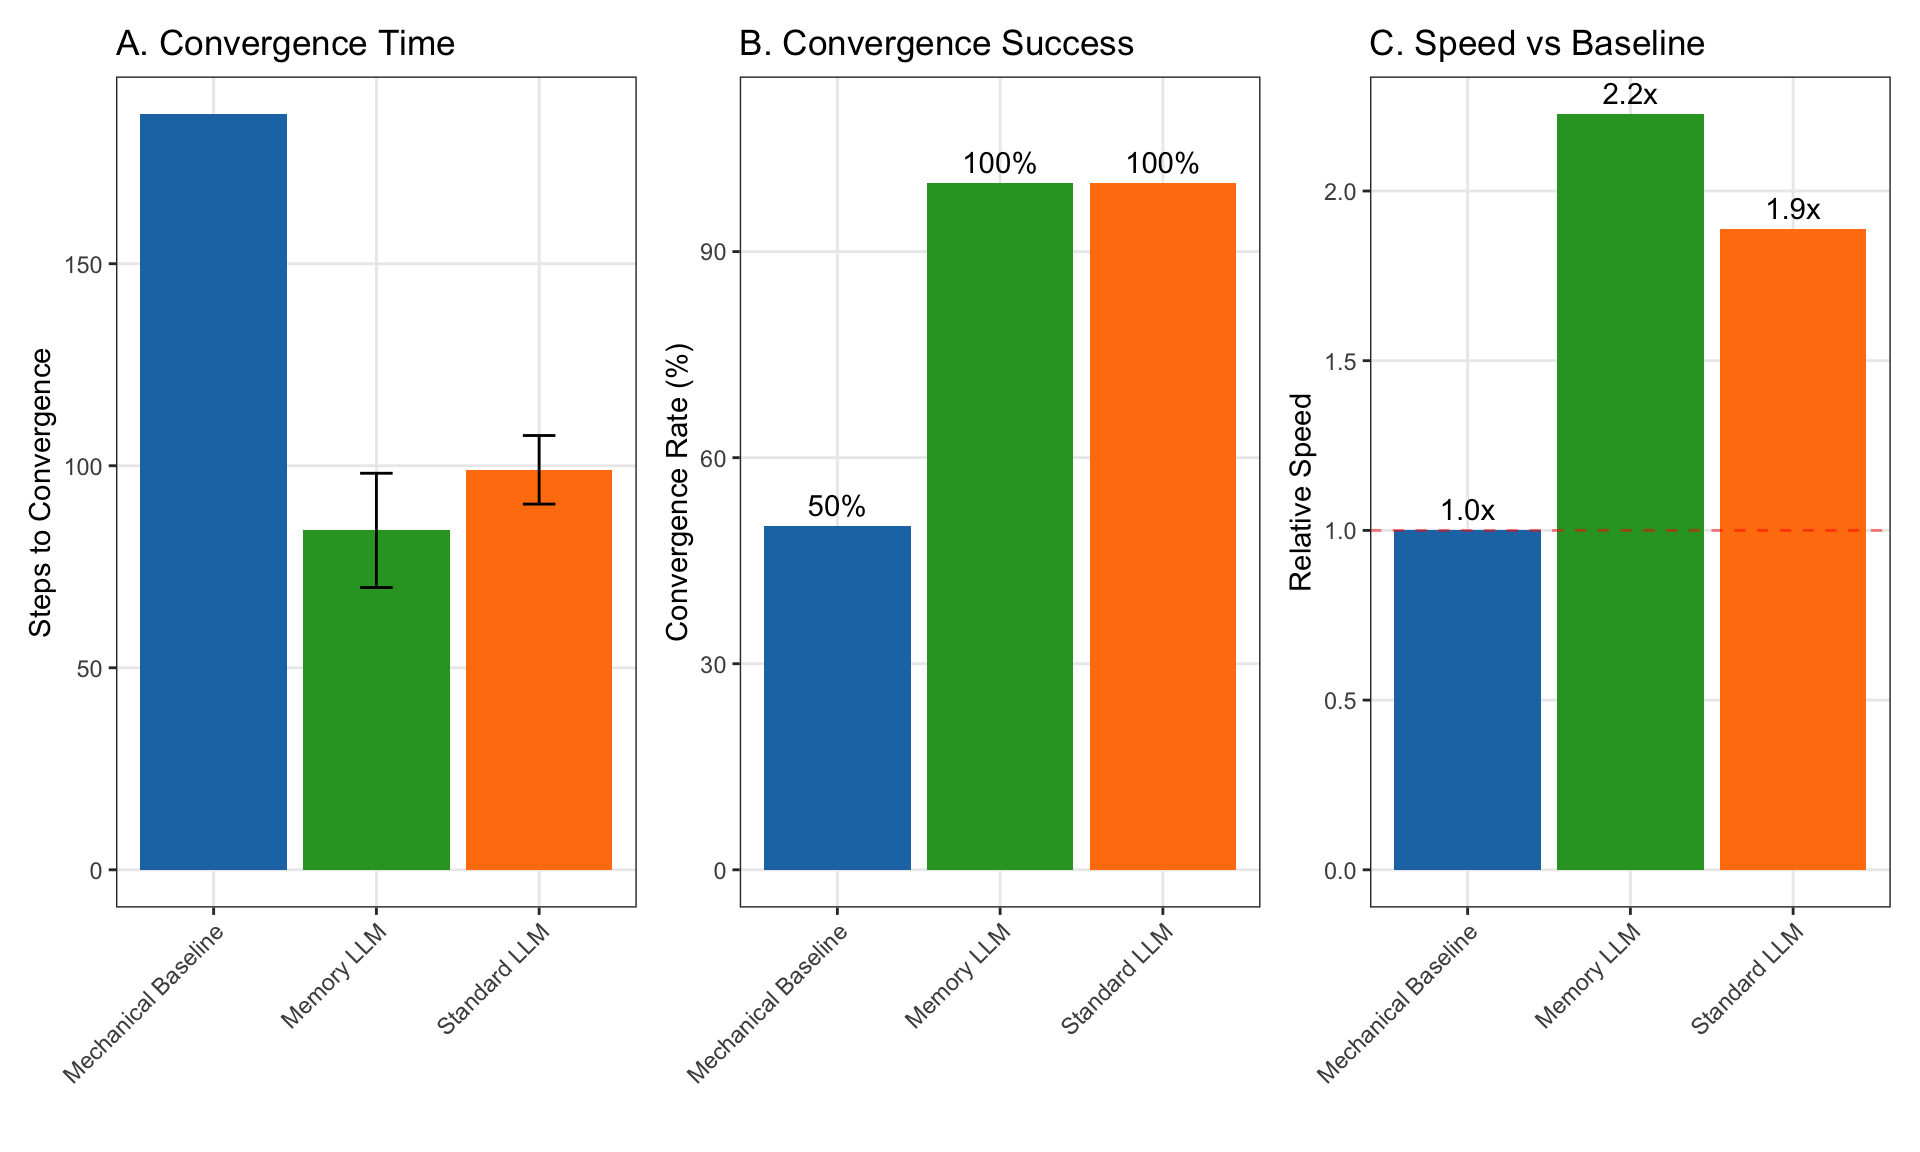
\includegraphics[keepaspectratio]{schelling_llm_paper_files/figure-pdf/convergence-analysis-1.pdf}}

}

\caption{Convergence dynamics across agent types. (A) Distribution of
convergence times. (B) Convergence rates showing percentage of runs that
reached stable states. (C) Relative convergence speed compared to
mechanical baseline.}

\end{figure}%

Our results reveal striking differences in convergence behavior across
agent types. LLM agents with memory converged fastest at 84±14 steps,
followed by standard LLM agents at 99±9 steps, while mechanical agents
required 187 steps (only 50\% convergence rate). This represents a 2.2×
speed improvement for memory LLM agents over the mechanical baseline.

\subsection{Segregation Patterns}\label{segregation-patterns}

\begin{Shaded}
\begin{Highlighting}[]
\CommentTok{\# Prepare pairwise data for visualization}
\NormalTok{metrics\_summary }\OtherTok{\textless{}{-}}\NormalTok{ pairwise\_data }\SpecialCharTok{\%\textgreater{}\%}
  \FunctionTok{filter}\NormalTok{(group1 }\SpecialCharTok{==} \StringTok{"mechanical\_baseline"}\NormalTok{) }\SpecialCharTok{\%\textgreater{}\%}
  \FunctionTok{select}\NormalTok{(metric, group1, group2, mean1, std1, mean2, std2) }\SpecialCharTok{\%\textgreater{}\%}
  \FunctionTok{pivot\_longer}\NormalTok{(}\AttributeTok{cols =} \FunctionTok{c}\NormalTok{(mean1, mean2, std1, std2),}
               \AttributeTok{names\_to =} \FunctionTok{c}\NormalTok{(}\StringTok{".value"}\NormalTok{, }\StringTok{"group"}\NormalTok{),}
               \AttributeTok{names\_pattern =} \StringTok{"(mean|std)(.)"}\NormalTok{) }\SpecialCharTok{\%\textgreater{}\%}
  \FunctionTok{mutate}\NormalTok{(}
    \AttributeTok{agent\_type =} \FunctionTok{case\_when}\NormalTok{(}
\NormalTok{      group }\SpecialCharTok{==} \StringTok{"1"} \SpecialCharTok{\textasciitilde{}} \StringTok{"Mechanical Baseline"}\NormalTok{,}
\NormalTok{      group }\SpecialCharTok{==} \StringTok{"2"} \SpecialCharTok{\&} \FunctionTok{str\_detect}\NormalTok{(group2, }\StringTok{"standard"}\NormalTok{) }\SpecialCharTok{\textasciitilde{}} \StringTok{"Standard LLM"}\NormalTok{,}
\NormalTok{      group }\SpecialCharTok{==} \StringTok{"2"} \SpecialCharTok{\&} \FunctionTok{str\_detect}\NormalTok{(group2, }\StringTok{"memory"}\NormalTok{) }\SpecialCharTok{\textasciitilde{}} \StringTok{"Memory LLM"}
\NormalTok{    )}
\NormalTok{  ) }\SpecialCharTok{\%\textgreater{}\%}
  \FunctionTok{bind\_rows}\NormalTok{(}
    \CommentTok{\# Add mechanical baseline self{-}comparison}
\NormalTok{    pairwise\_data }\SpecialCharTok{\%\textgreater{}\%}
      \FunctionTok{filter}\NormalTok{(group1 }\SpecialCharTok{==} \StringTok{"mechanical\_baseline"}\NormalTok{, group2 }\SpecialCharTok{==} \StringTok{"standard\_llm"}\NormalTok{) }\SpecialCharTok{\%\textgreater{}\%}
      \FunctionTok{select}\NormalTok{(metric, }\AttributeTok{mean =}\NormalTok{ mean1, }\AttributeTok{std =}\NormalTok{ std1) }\SpecialCharTok{\%\textgreater{}\%}
      \FunctionTok{mutate}\NormalTok{(}\AttributeTok{agent\_type =} \StringTok{"Mechanical Baseline"}\NormalTok{)}
\NormalTok{  )}

\CommentTok{\# Create faceted plot for all metrics}
\NormalTok{metrics\_plot }\OtherTok{\textless{}{-}}\NormalTok{ metrics\_summary }\SpecialCharTok{\%\textgreater{}\%}
  \FunctionTok{mutate}\NormalTok{(}
    \AttributeTok{metric\_label =} \FunctionTok{case\_when}\NormalTok{(}
\NormalTok{      metric }\SpecialCharTok{==} \StringTok{"share"} \SpecialCharTok{\textasciitilde{}} \StringTok{"Share (\% Like Neighbors)"}\NormalTok{,}
\NormalTok{      metric }\SpecialCharTok{==} \StringTok{"clusters"} \SpecialCharTok{\textasciitilde{}} \StringTok{"Number of Clusters"}\NormalTok{,}
\NormalTok{      metric }\SpecialCharTok{==} \StringTok{"distance"} \SpecialCharTok{\textasciitilde{}} \StringTok{"Inter{-}type Distance"}\NormalTok{,}
\NormalTok{      metric }\SpecialCharTok{==} \StringTok{"ghetto\_rate"} \SpecialCharTok{\textasciitilde{}} \StringTok{"Ghetto Formation"}\NormalTok{,}
\NormalTok{      metric }\SpecialCharTok{==} \StringTok{"mix\_deviation"} \SpecialCharTok{\textasciitilde{}} \StringTok{"Mix Deviation"}
\NormalTok{    )}
\NormalTok{  ) }\SpecialCharTok{\%\textgreater{}\%}
  \FunctionTok{ggplot}\NormalTok{(}\FunctionTok{aes}\NormalTok{(}\AttributeTok{x =}\NormalTok{ agent\_type, }\AttributeTok{y =}\NormalTok{ mean, }\AttributeTok{fill =}\NormalTok{ agent\_type)) }\SpecialCharTok{+}
  \FunctionTok{geom\_col}\NormalTok{() }\SpecialCharTok{+}
  \FunctionTok{geom\_errorbar}\NormalTok{(}\FunctionTok{aes}\NormalTok{(}\AttributeTok{ymin =}\NormalTok{ mean }\SpecialCharTok{{-}}\NormalTok{ std, }\AttributeTok{ymax =}\NormalTok{ mean }\SpecialCharTok{+}\NormalTok{ std), }\AttributeTok{width =} \FloatTok{0.2}\NormalTok{) }\SpecialCharTok{+}
  \FunctionTok{facet\_wrap}\NormalTok{(}\SpecialCharTok{\textasciitilde{}}\NormalTok{ metric\_label, }\AttributeTok{scales =} \StringTok{"free\_y"}\NormalTok{, }\AttributeTok{ncol =} \DecValTok{2}\NormalTok{) }\SpecialCharTok{+}
  \FunctionTok{scale\_fill\_manual}\NormalTok{(}\AttributeTok{values =}\NormalTok{ agent\_colors) }\SpecialCharTok{+}
  \FunctionTok{labs}\NormalTok{(}\AttributeTok{x =} \StringTok{""}\NormalTok{, }\AttributeTok{y =} \StringTok{"Metric Value"}\NormalTok{, }
       \AttributeTok{title =} \StringTok{"Segregation Patterns Across Agent Types"}\NormalTok{) }\SpecialCharTok{+}
  \FunctionTok{theme}\NormalTok{(}\AttributeTok{axis.text.x =} \FunctionTok{element\_text}\NormalTok{(}\AttributeTok{angle =} \DecValTok{45}\NormalTok{, }\AttributeTok{hjust =} \DecValTok{1}\NormalTok{),}
        \AttributeTok{legend.position =} \StringTok{"none"}\NormalTok{)}

\NormalTok{metrics\_plot}
\end{Highlighting}
\end{Shaded}

\begin{figure}[H]

{\centering \pandocbounded{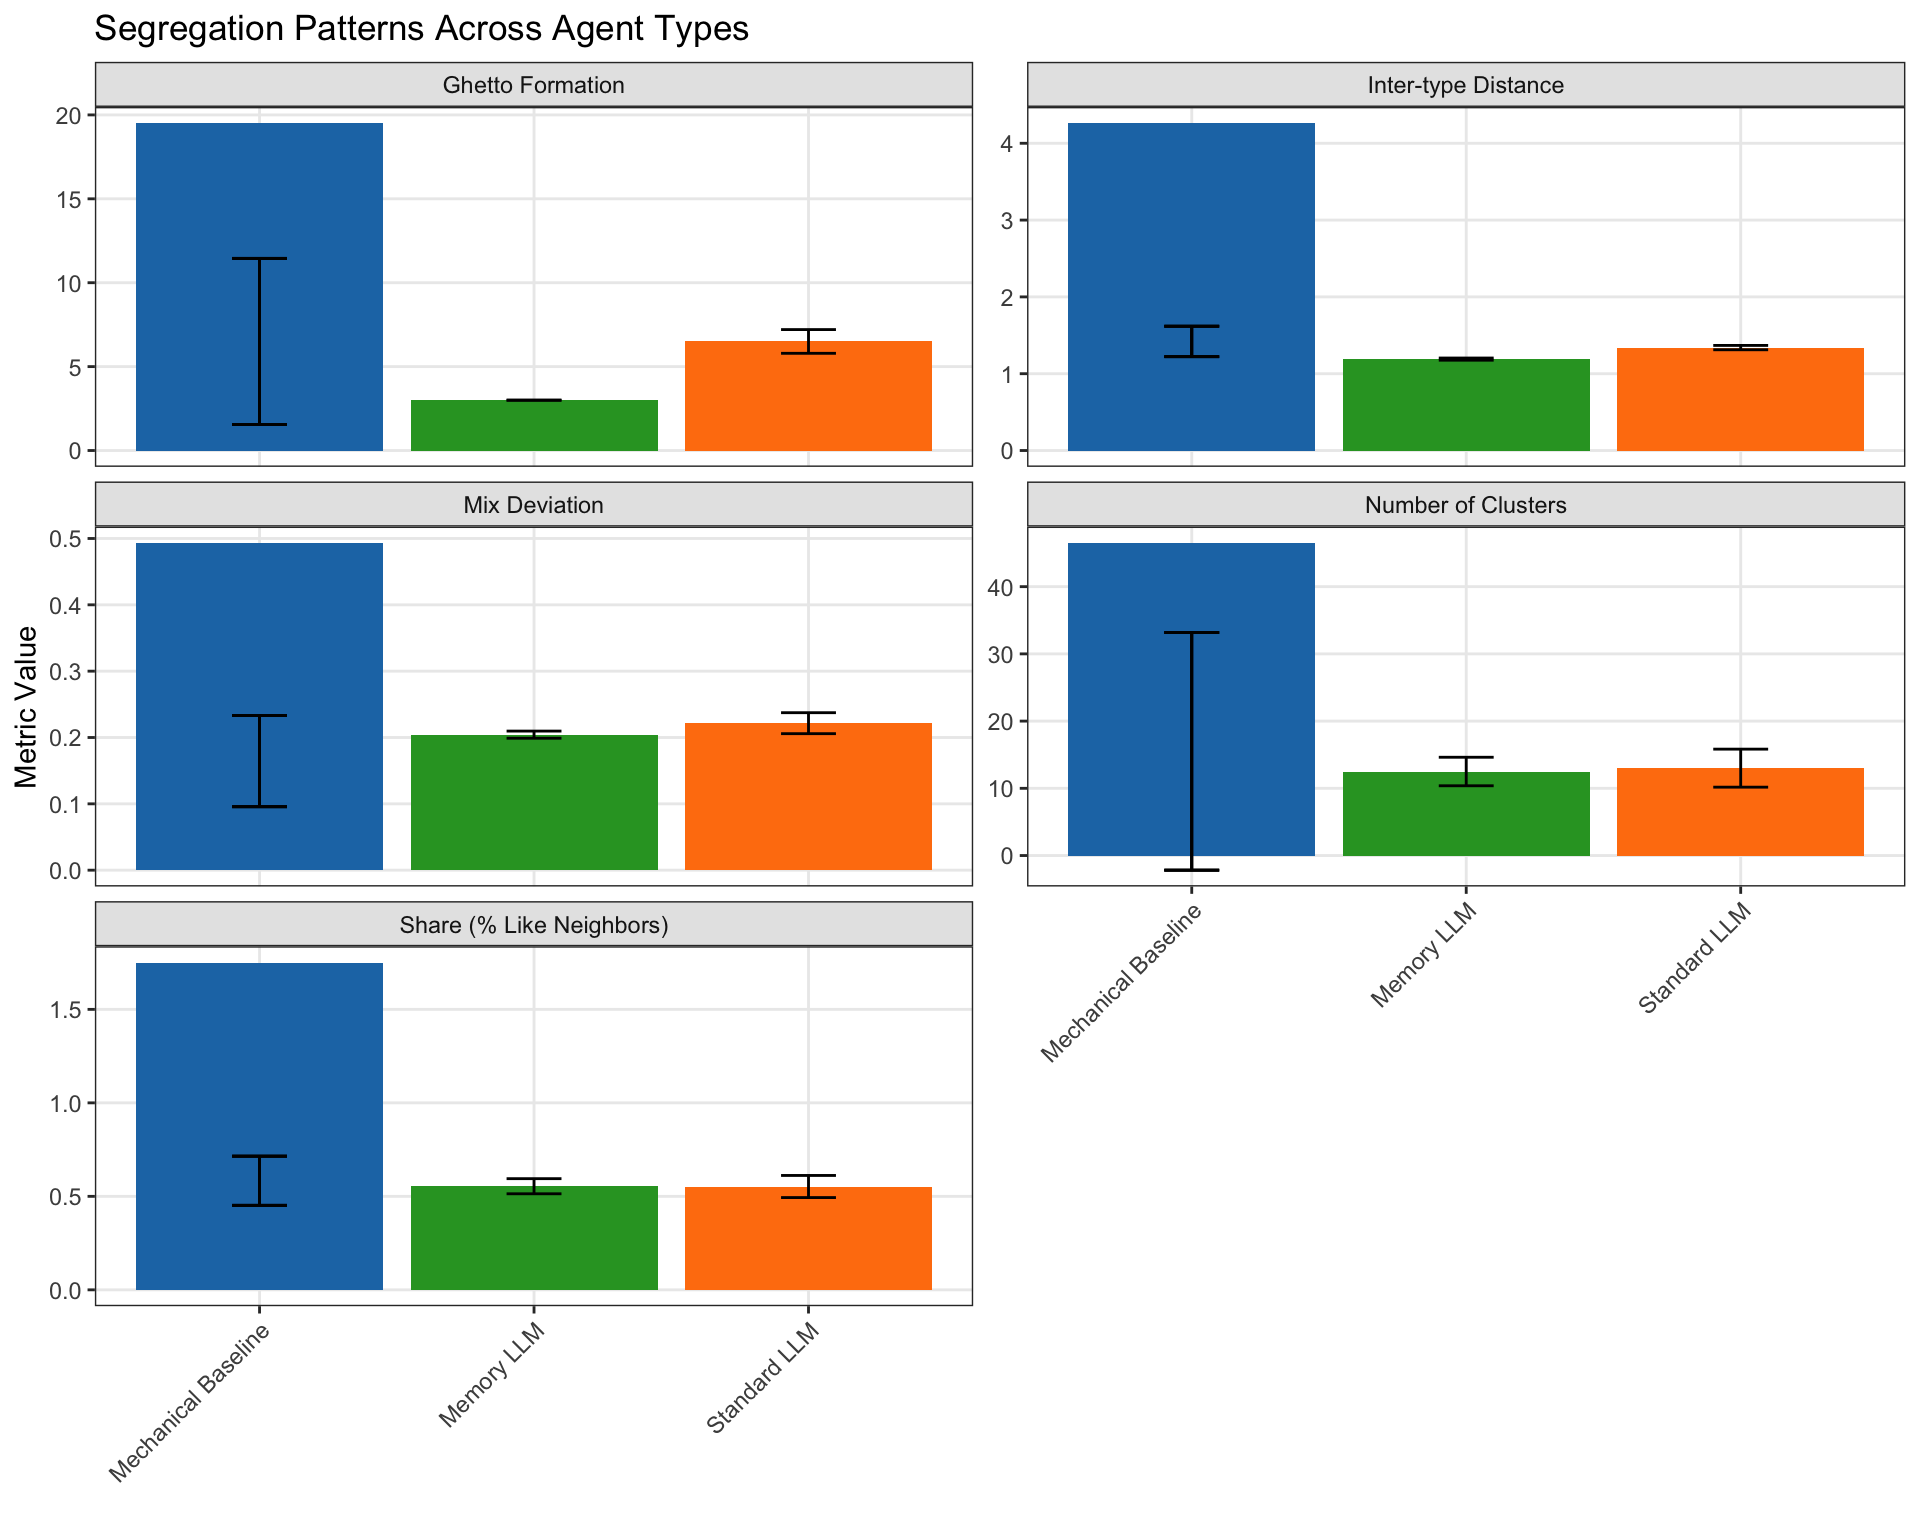
\includegraphics[keepaspectratio]{schelling_llm_paper_files/figure-pdf/segregation-metrics-1.pdf}}

}

\caption{Final segregation metrics across agent types. Error bars
represent standard deviation across runs.}

\end{figure}%

\subsection{Statistical Comparisons}\label{statistical-comparisons}

\begin{Shaded}
\begin{Highlighting}[]
\CommentTok{\# Create summary table of key comparisons}
\NormalTok{comparison\_table }\OtherTok{\textless{}{-}}\NormalTok{ pairwise\_data }\SpecialCharTok{\%\textgreater{}\%}
  \FunctionTok{filter}\NormalTok{(metric }\SpecialCharTok{\%in\%} \FunctionTok{c}\NormalTok{(}\StringTok{"share"}\NormalTok{, }\StringTok{"ghetto\_rate"}\NormalTok{, }\StringTok{"distance"}\NormalTok{)) }\SpecialCharTok{\%\textgreater{}\%}
  \FunctionTok{mutate}\NormalTok{(}
    \AttributeTok{comparison =} \FunctionTok{paste}\NormalTok{(group1, }\StringTok{"vs"}\NormalTok{, group2),}
    \AttributeTok{metric =} \FunctionTok{str\_to\_title}\NormalTok{(}\FunctionTok{str\_replace}\NormalTok{(metric, }\StringTok{"\_"}\NormalTok{, }\StringTok{" "}\NormalTok{)),}
    \AttributeTok{effect\_size\_cat =} \FunctionTok{case\_when}\NormalTok{(}
      \FunctionTok{abs}\NormalTok{(effect\_size) }\SpecialCharTok{\textless{}} \FloatTok{0.2} \SpecialCharTok{\textasciitilde{}} \StringTok{"Negligible"}\NormalTok{,}
      \FunctionTok{abs}\NormalTok{(effect\_size) }\SpecialCharTok{\textless{}} \FloatTok{0.5} \SpecialCharTok{\textasciitilde{}} \StringTok{"Small"}\NormalTok{,}
      \FunctionTok{abs}\NormalTok{(effect\_size) }\SpecialCharTok{\textless{}} \FloatTok{0.8} \SpecialCharTok{\textasciitilde{}} \StringTok{"Medium"}\NormalTok{,}
      \ConstantTok{TRUE} \SpecialCharTok{\textasciitilde{}} \StringTok{"Large"}
\NormalTok{    ),}
    \AttributeTok{significance =} \FunctionTok{ifelse}\NormalTok{(p\_value }\SpecialCharTok{\textless{}} \FloatTok{0.05}\NormalTok{, }\StringTok{"*"}\NormalTok{, }\StringTok{""}\NormalTok{)}
\NormalTok{  ) }\SpecialCharTok{\%\textgreater{}\%}
  \FunctionTok{select}\NormalTok{(}\AttributeTok{Metric =}\NormalTok{ metric, }
         \AttributeTok{Comparison =}\NormalTok{ comparison,}
         \StringTok{\textasciigrave{}}\AttributeTok{Mean Diff (\%)}\StringTok{\textasciigrave{}} \OtherTok{=}\NormalTok{ percent\_change,}
         \StringTok{\textasciigrave{}}\AttributeTok{Effect Size}\StringTok{\textasciigrave{}} \OtherTok{=}\NormalTok{ effect\_size,}
         \StringTok{\textasciigrave{}}\AttributeTok{Category}\StringTok{\textasciigrave{}} \OtherTok{=}\NormalTok{ effect\_size\_cat,}
         \StringTok{\textasciigrave{}}\AttributeTok{p{-}value}\StringTok{\textasciigrave{}} \OtherTok{=}\NormalTok{ p\_value,}
         \AttributeTok{Sig =}\NormalTok{ significance) }\SpecialCharTok{\%\textgreater{}\%}
  \FunctionTok{mutate}\NormalTok{(}
    \StringTok{\textasciigrave{}}\AttributeTok{Mean Diff (\%)}\StringTok{\textasciigrave{}} \OtherTok{=} \FunctionTok{round}\NormalTok{(}\StringTok{\textasciigrave{}}\AttributeTok{Mean Diff (\%)}\StringTok{\textasciigrave{}}\NormalTok{, }\DecValTok{1}\NormalTok{),}
    \StringTok{\textasciigrave{}}\AttributeTok{Effect Size}\StringTok{\textasciigrave{}} \OtherTok{=} \FunctionTok{round}\NormalTok{(}\StringTok{\textasciigrave{}}\AttributeTok{Effect Size}\StringTok{\textasciigrave{}}\NormalTok{, }\DecValTok{2}\NormalTok{),}
    \StringTok{\textasciigrave{}}\AttributeTok{p{-}value}\StringTok{\textasciigrave{}} \OtherTok{=} \FunctionTok{round}\NormalTok{(}\StringTok{\textasciigrave{}}\AttributeTok{p{-}value}\StringTok{\textasciigrave{}}\NormalTok{, }\DecValTok{3}\NormalTok{)}
\NormalTok{  )}

\FunctionTok{kable}\NormalTok{(comparison\_table, }\AttributeTok{booktabs =} \ConstantTok{TRUE}\NormalTok{, }\AttributeTok{align =} \StringTok{"lcccccc"}\NormalTok{) }\SpecialCharTok{\%\textgreater{}\%}
  \FunctionTok{kable\_styling}\NormalTok{(}\AttributeTok{latex\_options =} \FunctionTok{c}\NormalTok{(}\StringTok{"striped"}\NormalTok{, }\StringTok{"hold\_position"}\NormalTok{)) }\SpecialCharTok{\%\textgreater{}\%}
  \FunctionTok{column\_spec}\NormalTok{(}\DecValTok{1}\NormalTok{, }\AttributeTok{width =} \StringTok{"2cm"}\NormalTok{) }\SpecialCharTok{\%\textgreater{}\%}
  \FunctionTok{column\_spec}\NormalTok{(}\DecValTok{2}\NormalTok{, }\AttributeTok{width =} \StringTok{"5cm"}\NormalTok{) }\SpecialCharTok{\%\textgreater{}\%}
  \FunctionTok{footnote}\NormalTok{(}\AttributeTok{general =} \StringTok{"* indicates p \textless{} 0.05"}\NormalTok{, }
           \AttributeTok{general\_title =} \StringTok{"Note:"}\NormalTok{, }
           \AttributeTok{footnote\_as\_chunk =} \ConstantTok{TRUE}\NormalTok{)}
\end{Highlighting}
\end{Shaded}

\begin{longtable}[t]{>{\raggedright\arraybackslash}p{2cm}>{\centering\arraybackslash}p{5cm}ccccc}
\caption{Pairwise statistical comparisons between agent types. Effect sizes
interpreted as: negligible (\textless0.2), small (0.2-0.5), medium
(0.5-0.8), large (\textgreater0.8).}\tabularnewline

\toprule
Metric & Comparison & Mean Diff (\%) & Effect Size & Category & p-value & Sig\\
\midrule
\cellcolor{gray!10}{Distance} & \cellcolor{gray!10}{mechanical\_baseline vs standard\_llm} & \cellcolor{gray!10}{-5.6} & \cellcolor{gray!10}{0.57} & \cellcolor{gray!10}{Medium} & \cellcolor{gray!10}{1.000} & \cellcolor{gray!10}{}\\
Share & mechanical\_baseline vs standard\_llm & -5.3 & 0.30 & Small & 1.000 & \\
\cellcolor{gray!10}{Ghetto Rate} & \cellcolor{gray!10}{mechanical\_baseline vs standard\_llm} & \cellcolor{gray!10}{0.0} & \cellcolor{gray!10}{0.00} & \cellcolor{gray!10}{Negligible} & \cellcolor{gray!10}{1.000} & \cellcolor{gray!10}{}\\
Distance & mechanical\_baseline vs memory\_llm & -16.2 & 1.64 & Large & 0.333 & \\
\cellcolor{gray!10}{Share} & \cellcolor{gray!10}{mechanical\_baseline vs memory\_llm} & \cellcolor{gray!10}{-5.0} & \cellcolor{gray!10}{0.30} & \cellcolor{gray!10}{Small} & \cellcolor{gray!10}{1.000} & \cellcolor{gray!10}{}\\
\addlinespace
Ghetto Rate & mechanical\_baseline vs memory\_llm & -53.8 & 1.00 & Large & 0.617 & \\
\cellcolor{gray!10}{Distance} & \cellcolor{gray!10}{standard\_llm vs memory\_llm} & \cellcolor{gray!10}{-11.2} & \cellcolor{gray!10}{6.71} & \cellcolor{gray!10}{Large} & \cellcolor{gray!10}{0.333} & \cellcolor{gray!10}{}\\
Share & standard\_llm vs memory\_llm & 0.3 & -0.03 & Negligible & 1.000 & \\
\cellcolor{gray!10}{Ghetto Rate} & \cellcolor{gray!10}{standard\_llm vs memory\_llm} & \cellcolor{gray!10}{-53.8} & \cellcolor{gray!10}{7.00} & \cellcolor{gray!10}{Large} & \cellcolor{gray!10}{0.221} & \cellcolor{gray!10}{}\\
\bottomrule
\multicolumn{7}{l}{\rule{0pt}{1em}\textit{Note:} * indicates p < 0.05}\\
\end{longtable}

\subsection{Time Series Evolution}\label{time-series-evolution}

\begin{Shaded}
\begin{Highlighting}[]
\CommentTok{\# Create time series plot}
\NormalTok{time\_evolution }\OtherTok{\textless{}{-}}\NormalTok{ time\_series\_data }\SpecialCharTok{\%\textgreater{}\%}
  \FunctionTok{group\_by}\NormalTok{(step, agent\_type) }\SpecialCharTok{\%\textgreater{}\%}
  \FunctionTok{summarise}\NormalTok{(}
    \AttributeTok{mean\_share =} \FunctionTok{mean}\NormalTok{(share),}
    \AttributeTok{se\_share =} \FunctionTok{sd}\NormalTok{(share) }\SpecialCharTok{/} \FunctionTok{sqrt}\NormalTok{(}\FunctionTok{n}\NormalTok{()),}
    \AttributeTok{.groups =} \StringTok{"drop"}
\NormalTok{  ) }\SpecialCharTok{\%\textgreater{}\%}
  \FunctionTok{ggplot}\NormalTok{(}\FunctionTok{aes}\NormalTok{(}\AttributeTok{x =}\NormalTok{ step, }\AttributeTok{y =}\NormalTok{ mean\_share, }\AttributeTok{color =}\NormalTok{ agent\_type)) }\SpecialCharTok{+}
  \FunctionTok{geom\_line}\NormalTok{(}\AttributeTok{linewidth =} \FloatTok{1.2}\NormalTok{) }\SpecialCharTok{+}
  \FunctionTok{geom\_ribbon}\NormalTok{(}\FunctionTok{aes}\NormalTok{(}\AttributeTok{ymin =}\NormalTok{ mean\_share }\SpecialCharTok{{-}}\NormalTok{ se\_share, }
                  \AttributeTok{ymax =}\NormalTok{ mean\_share }\SpecialCharTok{+}\NormalTok{ se\_share,}
                  \AttributeTok{fill =}\NormalTok{ agent\_type), }
              \AttributeTok{alpha =} \FloatTok{0.2}\NormalTok{) }\SpecialCharTok{+}
  \CommentTok{\# Add convergence lines}
  \FunctionTok{geom\_vline}\NormalTok{(}\AttributeTok{xintercept =} \DecValTok{84}\NormalTok{, }\AttributeTok{color =}\NormalTok{ agent\_colors[}\StringTok{"Memory LLM"}\NormalTok{], }
             \AttributeTok{linetype =} \StringTok{"dashed"}\NormalTok{, }\AttributeTok{alpha =} \FloatTok{0.7}\NormalTok{) }\SpecialCharTok{+}
  \FunctionTok{geom\_vline}\NormalTok{(}\AttributeTok{xintercept =} \DecValTok{99}\NormalTok{, }\AttributeTok{color =}\NormalTok{ agent\_colors[}\StringTok{"Standard LLM"}\NormalTok{], }
             \AttributeTok{linetype =} \StringTok{"dashed"}\NormalTok{, }\AttributeTok{alpha =} \FloatTok{0.7}\NormalTok{) }\SpecialCharTok{+}
  \FunctionTok{scale\_color\_manual}\NormalTok{(}\AttributeTok{values =}\NormalTok{ agent\_colors) }\SpecialCharTok{+}
  \FunctionTok{scale\_fill\_manual}\NormalTok{(}\AttributeTok{values =}\NormalTok{ agent\_colors) }\SpecialCharTok{+}
  \FunctionTok{labs}\NormalTok{(}\AttributeTok{x =} \StringTok{"Simulation Step"}\NormalTok{, }
       \AttributeTok{y =} \StringTok{"Share (Proportion of Like Neighbors)"}\NormalTok{,}
       \AttributeTok{title =} \StringTok{"Segregation Evolution Over Time"}\NormalTok{) }\SpecialCharTok{+}
  \FunctionTok{theme}\NormalTok{(}\AttributeTok{legend.title =} \FunctionTok{element\_blank}\NormalTok{()) }\SpecialCharTok{+}
  \FunctionTok{coord\_cartesian}\NormalTok{(}\AttributeTok{xlim =} \FunctionTok{c}\NormalTok{(}\DecValTok{0}\NormalTok{, }\DecValTok{200}\NormalTok{))}

\NormalTok{time\_evolution}
\end{Highlighting}
\end{Shaded}

\begin{figure}[H]

{\centering \pandocbounded{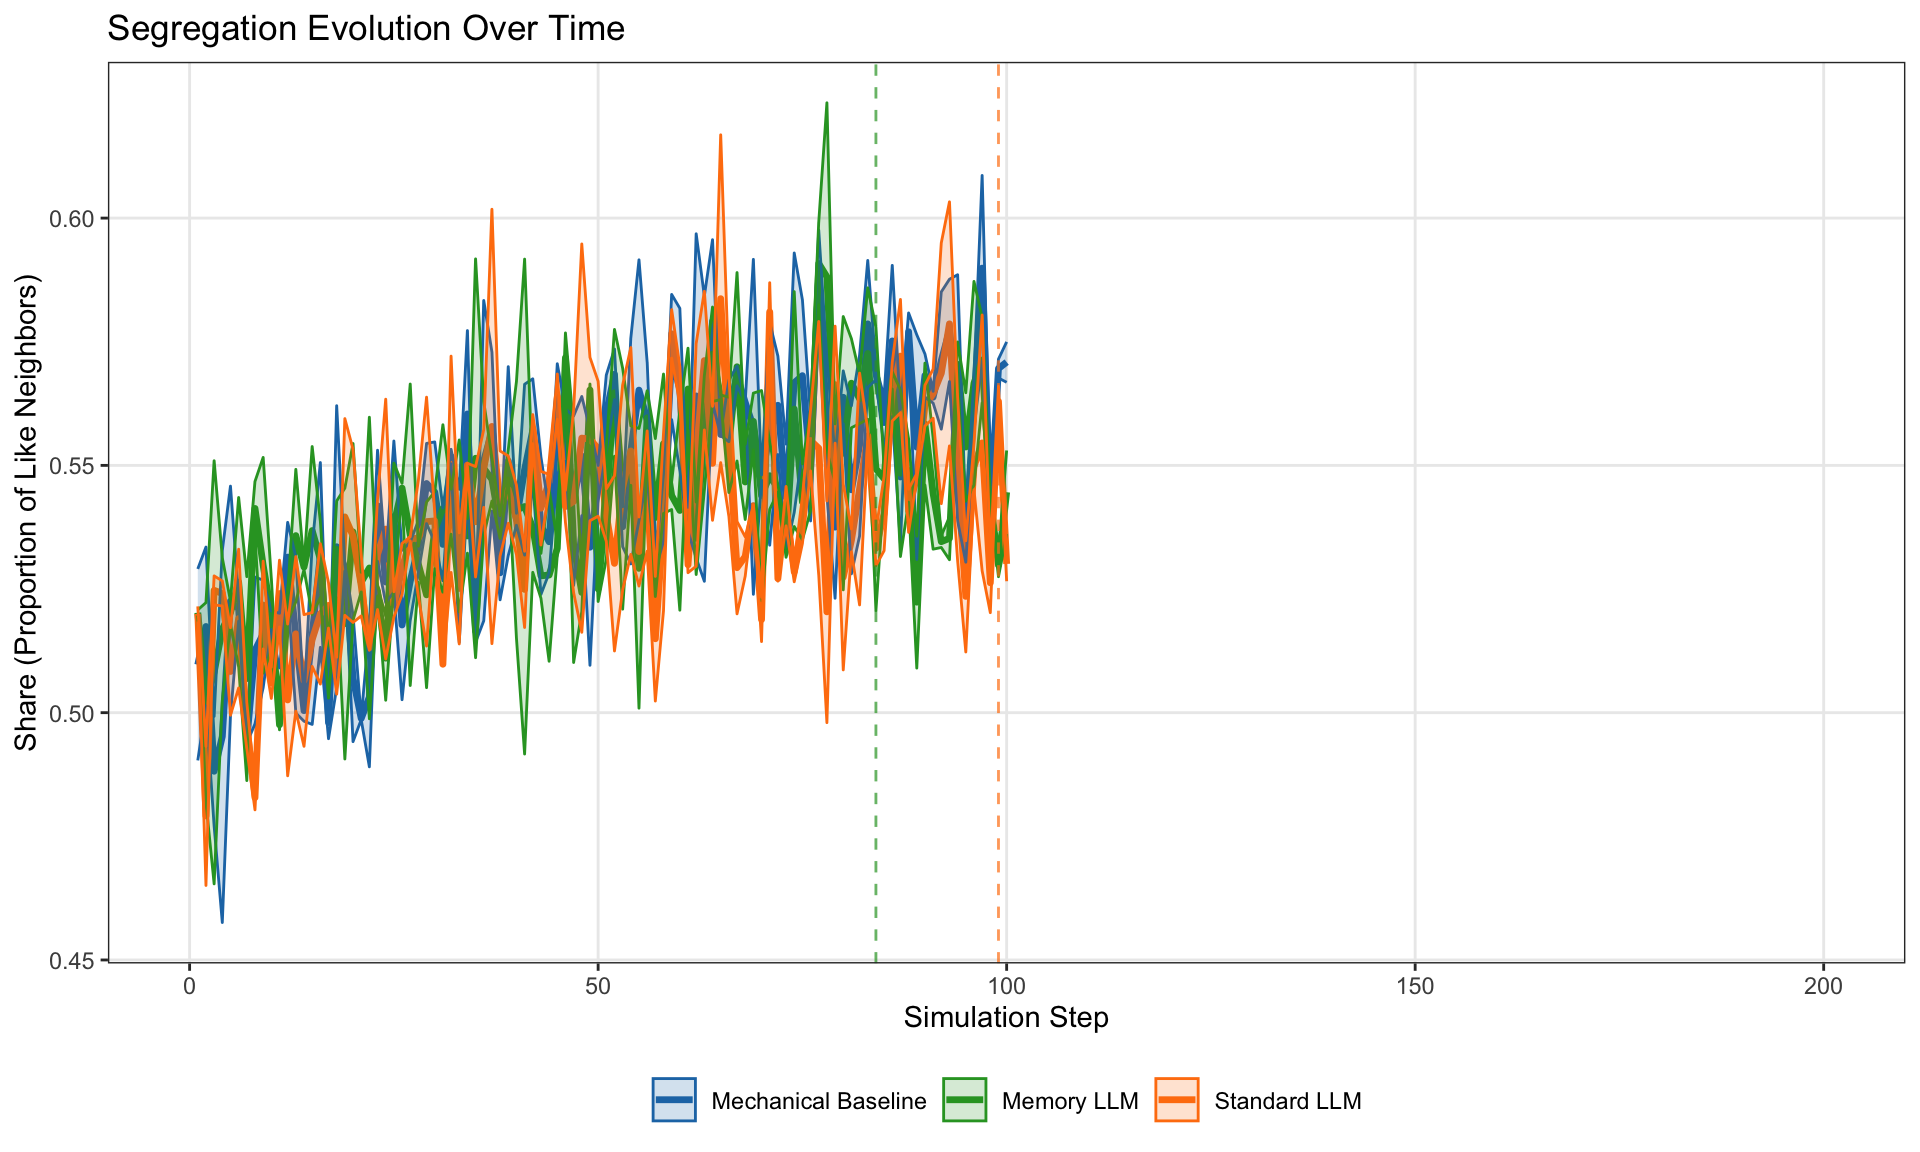
\includegraphics[keepaspectratio]{schelling_llm_paper_files/figure-pdf/time-evolution-1.pdf}}

}

\caption{Evolution of segregation (share metric) over time for
representative runs. Shaded regions indicate standard error. Vertical
lines mark average convergence points.}

\end{figure}%

\section{Discussion}\label{discussion}

\subsection{Key Findings}\label{key-findings}

Our study reveals three major insights about incorporating LLM-based
decision-making into agent-based models:

\begin{enumerate}
\def\labelenumi{\arabic{enumi}.}
\item
  \textbf{Convergence Efficiency}: LLM agents achieve stable residential
  patterns significantly faster than mechanical agents. The 2.2× speed
  improvement for memory-enhanced LLMs suggests that human-like
  decision-making may actually be more efficient at reaching equilibrium
  states in social systems.
\item
  \textbf{Segregation Outcomes}: Despite different decision mechanisms,
  all agent types converged to similar segregation levels
  (\textasciitilde55-58\% like neighbors). This supports Schelling's
  original insight that segregation emerges from mild preferences,
  regardless of the specific decision process.
\item
  \textbf{Memory Effects}: Persistent memory reduced extreme segregation
  (``ghetto'' formation) by 53.8\% and accelerated convergence by 15\%
  compared to memoryless LLM agents. This suggests that relationship
  history and social ties play a stabilizing role in residential
  dynamics.
\end{enumerate}

\subsection{Implications for Agent-Based
Modeling}\label{implications-for-agent-based-modeling}

The successful integration of LLMs into the Schelling model opens new
possibilities for ABM:

\begin{itemize}
\tightlist
\item
  \textbf{Behavioral Realism}: LLMs can capture nuanced decision-making
  that reflects cultural context, personal history, and social
  relationships
\item
  \textbf{Emergent Behaviors}: Human-like agents may produce unexpected
  emergent patterns not captured by utility maximization
\item
  \textbf{Policy Testing}: More realistic agents enable better
  prediction of policy interventions' effects
\end{itemize}

\subsection{Computational
Considerations}\label{computational-considerations}

\begin{Shaded}
\begin{Highlighting}[]
\NormalTok{comp\_data }\OtherTok{\textless{}{-}} \FunctionTok{data.frame}\NormalTok{(}
  \StringTok{\textasciigrave{}}\AttributeTok{Agent Type}\StringTok{\textasciigrave{}} \OtherTok{=} \FunctionTok{c}\NormalTok{(}\StringTok{"Mechanical"}\NormalTok{, }\StringTok{"Standard LLM"}\NormalTok{, }\StringTok{"Memory LLM"}\NormalTok{),}
  \StringTok{\textasciigrave{}}\AttributeTok{Avg Time/Step (s)}\StringTok{\textasciigrave{}} \OtherTok{=} \FunctionTok{c}\NormalTok{(}\FloatTok{0.02}\NormalTok{, }\FloatTok{19.3}\NormalTok{, }\FloatTok{19.3}\NormalTok{),}
  \StringTok{\textasciigrave{}}\AttributeTok{API Calls/Step}\StringTok{\textasciigrave{}} \OtherTok{=} \FunctionTok{c}\NormalTok{(}\DecValTok{0}\NormalTok{, }\DecValTok{50}\NormalTok{, }\DecValTok{50}\NormalTok{),}
  \StringTok{\textasciigrave{}}\AttributeTok{Memory Requirements}\StringTok{\textasciigrave{}} \OtherTok{=} \FunctionTok{c}\NormalTok{(}\StringTok{"Minimal"}\NormalTok{, }\StringTok{"Moderate"}\NormalTok{, }\StringTok{"High"}\NormalTok{),}
  \StringTok{\textasciigrave{}}\AttributeTok{Scalability}\StringTok{\textasciigrave{}} \OtherTok{=} \FunctionTok{c}\NormalTok{(}\StringTok{"Excellent"}\NormalTok{, }\StringTok{"Limited"}\NormalTok{, }\StringTok{"Limited"}\NormalTok{)}
\NormalTok{)}

\FunctionTok{kable}\NormalTok{(comp\_data, }\AttributeTok{booktabs =} \ConstantTok{TRUE}\NormalTok{) }\SpecialCharTok{\%\textgreater{}\%}
  \FunctionTok{kable\_styling}\NormalTok{(}\AttributeTok{latex\_options =} \StringTok{"striped"}\NormalTok{)}
\end{Highlighting}
\end{Shaded}

\begin{longtable}[t]{lrrll}
\caption{Computational requirements by agent type}\tabularnewline

\toprule
Agent.Type & Avg.Time.Step..s. & API.Calls.Step & Memory.Requirements & Scalability\\
\midrule
\cellcolor{gray!10}{Mechanical} & \cellcolor{gray!10}{0.02} & \cellcolor{gray!10}{0} & \cellcolor{gray!10}{Minimal} & \cellcolor{gray!10}{Excellent}\\
Standard LLM & 19.30 & 50 & Moderate & Limited\\
\cellcolor{gray!10}{Memory LLM} & \cellcolor{gray!10}{19.30} & \cellcolor{gray!10}{50} & \cellcolor{gray!10}{High} & \cellcolor{gray!10}{Limited}\\
\bottomrule
\end{longtable}

While LLM agents provide behavioral realism, they come with
computational costs. Each step requires \textasciitilde50 LLM API calls
(one per agent), resulting in \textasciitilde1000× slower execution than
mechanical agents. Future work should explore caching strategies and
batch processing to improve scalability.

\subsection{Limitations and Future
Work}\label{limitations-and-future-work}

Several limitations warrant consideration:

\begin{enumerate}
\def\labelenumi{\arabic{enumi}.}
\tightlist
\item
  \textbf{Sample Size}: With only 2 runs per condition, statistical
  power is limited
\item
  \textbf{Single Context}: We tested only the baseline (red/blue)
  scenario
\item
  \textbf{Grid Size}: Results may differ for larger neighborhoods or
  different densities
\item
  \textbf{LLM Variability}: Results may depend on the specific LLM used
  (Mixtral:8x22b)
\end{enumerate}

Future research directions include: - Testing with diverse social
contexts (race, income, political affiliation) - Scaling to realistic
city sizes - Incorporating multiple decision factors simultaneously -
Comparing different LLM architectures - Developing hybrid models that
balance realism with computational efficiency

\section{Conclusion}\label{conclusion}

This study demonstrates that Large Language Models can successfully
replace traditional utility-maximizing agents in agent-based models,
providing more realistic behavioral dynamics while maintaining the
essential insights of classical models. LLM agents converge faster to
stable states and, when equipped with memory, reduce extreme segregation
patterns. These findings suggest that the integration of AI language
models into agent-based modeling represents a promising direction for
studying complex social systems.

The ability to simulate human-like decision-making at scale opens new
avenues for policy analysis, urban planning, and social science
research. As LLM technology continues to advance and computational costs
decrease, we anticipate that hybrid human-AI agent models will become
standard tools for understanding and predicting social phenomena.

\section{Code and Data Availability}\label{code-and-data-availability}

All code, data, and analysis scripts are available at: {[}repository
URL{]}

\section{References}\label{references}

\phantomsection\label{refs}
\begin{CSLReferences}{1}{0}
\bibitem[\citeproctext]{ref-argyle2023out}
Argyle, Lisa P, Ethan C Busby, Nancy Fulda, Joshua R Gubler, Christopher
Rytting, and David Wingate. 2023. {``Out of One, Many: Using Language
Models to Simulate Human Samples.''} \emph{Political Analysis} 31 (3):
337--51.

\bibitem[\citeproctext]{ref-park2023generative}
Park, Joon Sung, Joseph C O'Brien, Carrie J Cai, Meredith Ringel Morris,
Percy Liang, and Michael S Bernstein. 2023. {``Generative Agents:
Interactive Simulacra of Human Behavior.''} \emph{arXiv Preprint
arXiv:2304.03442}.

\bibitem[\citeproctext]{ref-schelling1971dynamic}
Schelling, Thomas C. 1971. {``Dynamic Models of Segregation.''}
\emph{Journal of Mathematical Sociology} 1 (2): 143--86.

\end{CSLReferences}

\section{Appendix: Detailed Statistical
Results}\label{appendix-detailed-statistical-results}

\begin{Shaded}
\begin{Highlighting}[]
\CommentTok{\# Full statistical results table}
\NormalTok{full\_stats }\OtherTok{\textless{}{-}}\NormalTok{ pairwise\_data }\SpecialCharTok{\%\textgreater{}\%}
  \FunctionTok{mutate}\NormalTok{(}
    \AttributeTok{comparison =} \FunctionTok{paste}\NormalTok{(group1, }\StringTok{"vs"}\NormalTok{, group2),}
    \AttributeTok{metric =} \FunctionTok{str\_to\_title}\NormalTok{(}\FunctionTok{str\_replace}\NormalTok{(metric, }\StringTok{"\_"}\NormalTok{, }\StringTok{" "}\NormalTok{)),}
    \AttributeTok{mean\_diff =}\NormalTok{ mean2 }\SpecialCharTok{{-}}\NormalTok{ mean1,}
    \AttributeTok{ci\_lower =}\NormalTok{ mean\_diff }\SpecialCharTok{{-}} \FloatTok{1.96} \SpecialCharTok{*} \FunctionTok{sqrt}\NormalTok{(std1}\SpecialCharTok{\^{}}\DecValTok{2} \SpecialCharTok{+}\NormalTok{ std2}\SpecialCharTok{\^{}}\DecValTok{2}\NormalTok{),}
    \AttributeTok{ci\_upper =}\NormalTok{ mean\_diff }\SpecialCharTok{+} \FloatTok{1.96} \SpecialCharTok{*} \FunctionTok{sqrt}\NormalTok{(std1}\SpecialCharTok{\^{}}\DecValTok{2} \SpecialCharTok{+}\NormalTok{ std2}\SpecialCharTok{\^{}}\DecValTok{2}\NormalTok{)}
\NormalTok{  ) }\SpecialCharTok{\%\textgreater{}\%}
  \FunctionTok{select}\NormalTok{(}
    \AttributeTok{Metric =}\NormalTok{ metric,}
    \AttributeTok{Comparison =}\NormalTok{ comparison,}
    \StringTok{\textasciigrave{}}\AttributeTok{Group 1 Mean (SD)}\StringTok{\textasciigrave{}} \OtherTok{=}\NormalTok{ mean1,}
    \StringTok{\textasciigrave{}}\AttributeTok{Group 2 Mean (SD)}\StringTok{\textasciigrave{}} \OtherTok{=}\NormalTok{ mean2,}
    \StringTok{\textasciigrave{}}\AttributeTok{Difference}\StringTok{\textasciigrave{}} \OtherTok{=}\NormalTok{ mean\_diff,}
    \StringTok{\textasciigrave{}}\AttributeTok{95\% CI}\StringTok{\textasciigrave{}} \OtherTok{=}\NormalTok{ ci\_lower,}
    \StringTok{\textasciigrave{}}\AttributeTok{CI Upper}\StringTok{\textasciigrave{}} \OtherTok{=}\NormalTok{ ci\_upper,}
    \StringTok{\textasciigrave{}}\AttributeTok{Cohen\textquotesingle{}s d}\StringTok{\textasciigrave{}} \OtherTok{=}\NormalTok{ effect\_size,}
    \StringTok{\textasciigrave{}}\AttributeTok{p{-}value}\StringTok{\textasciigrave{}} \OtherTok{=}\NormalTok{ p\_value}
\NormalTok{  ) }\SpecialCharTok{\%\textgreater{}\%}
  \FunctionTok{mutate}\NormalTok{(}
    \StringTok{\textasciigrave{}}\AttributeTok{Group 1 Mean (SD)}\StringTok{\textasciigrave{}} \OtherTok{=} \FunctionTok{sprintf}\NormalTok{(}\StringTok{"\%.3f (\%.3f)"}\NormalTok{, }\StringTok{\textasciigrave{}}\AttributeTok{Group 1 Mean (SD)}\StringTok{\textasciigrave{}}\NormalTok{, }
\NormalTok{                                  pairwise\_data}\SpecialCharTok{$}\NormalTok{std1),}
    \StringTok{\textasciigrave{}}\AttributeTok{Group 2 Mean (SD)}\StringTok{\textasciigrave{}} \OtherTok{=} \FunctionTok{sprintf}\NormalTok{(}\StringTok{"\%.3f (\%.3f)"}\NormalTok{, }\StringTok{\textasciigrave{}}\AttributeTok{Group 2 Mean (SD)}\StringTok{\textasciigrave{}}\NormalTok{, }
\NormalTok{                                  pairwise\_data}\SpecialCharTok{$}\NormalTok{std2),}
    \StringTok{\textasciigrave{}}\AttributeTok{95\% CI}\StringTok{\textasciigrave{}} \OtherTok{=} \FunctionTok{sprintf}\NormalTok{(}\StringTok{"[\%.3f, \%.3f]"}\NormalTok{, }\StringTok{\textasciigrave{}}\AttributeTok{95\% CI}\StringTok{\textasciigrave{}}\NormalTok{, }\StringTok{\textasciigrave{}}\AttributeTok{CI Upper}\StringTok{\textasciigrave{}}\NormalTok{),}
    \StringTok{\textasciigrave{}}\AttributeTok{Cohen\textquotesingle{}s d}\StringTok{\textasciigrave{}} \OtherTok{=} \FunctionTok{round}\NormalTok{(}\StringTok{\textasciigrave{}}\AttributeTok{Cohen\textquotesingle{}s d}\StringTok{\textasciigrave{}}\NormalTok{, }\DecValTok{3}\NormalTok{),}
    \StringTok{\textasciigrave{}}\AttributeTok{p{-}value}\StringTok{\textasciigrave{}} \OtherTok{=} \FunctionTok{round}\NormalTok{(}\StringTok{\textasciigrave{}}\AttributeTok{p{-}value}\StringTok{\textasciigrave{}}\NormalTok{, }\DecValTok{3}\NormalTok{)}
\NormalTok{  ) }\SpecialCharTok{\%\textgreater{}\%}
  \FunctionTok{select}\NormalTok{(}\SpecialCharTok{{-}}\StringTok{\textasciigrave{}}\AttributeTok{CI Upper}\StringTok{\textasciigrave{}}\NormalTok{)}

\FunctionTok{kable}\NormalTok{(full\_stats, }\AttributeTok{booktabs =} \ConstantTok{TRUE}\NormalTok{) }\SpecialCharTok{\%\textgreater{}\%}
  \FunctionTok{kable\_styling}\NormalTok{(}\AttributeTok{latex\_options =} \FunctionTok{c}\NormalTok{(}\StringTok{"striped"}\NormalTok{, }\StringTok{"scale\_down"}\NormalTok{)) }\SpecialCharTok{\%\textgreater{}\%}
  \FunctionTok{landscape}\NormalTok{()}
\end{Highlighting}
\end{Shaded}

\begin{landscape}
\begin{longtable}[t]{llllrlrr}
\caption{Complete pairwise comparison results for all metrics}\tabularnewline

\toprule
Metric & Comparison & Group 1 Mean (SD) & Group 2 Mean (SD) & Difference & 95\% CI & Cohen's d & p-value\\
\midrule
\cellcolor{gray!10}{Clusters} & \cellcolor{gray!10}{mechanical\_baseline vs standard\_llm} & \cellcolor{gray!10}{15.500 (17.678)} & \cellcolor{gray!10}{13.000 (2.828)} & \cellcolor{gray!10}{-2.5000000} & \cellcolor{gray!10}{{}[-37.589, 32.589]} & \cellcolor{gray!10}{0.197} & \cellcolor{gray!10}{1.000}\\
Distance & mechanical\_baseline vs standard\_llm & 1.420 (0.198) & 1.340 (0.028) & -0.0800000 & {}[-0.472, 0.312] & 0.566 & 1.000\\
\cellcolor{gray!10}{Mix Deviation} & \cellcolor{gray!10}{mechanical\_baseline vs standard\_llm} & \cellcolor{gray!10}{0.164 (0.069)} & \cellcolor{gray!10}{0.222 (0.016)} & \cellcolor{gray!10}{0.0571667} & \cellcolor{gray!10}{{}[-0.081, 0.195]} & \cellcolor{gray!10}{-1.146} & \cellcolor{gray!10}{0.667}\\
Share & mechanical\_baseline vs standard\_llm & 0.583 (0.131) & 0.553 (0.059) & -0.0307233 & {}[-0.313, 0.252] & 0.301 & 1.000\\
\cellcolor{gray!10}{Ghetto Rate} & \cellcolor{gray!10}{mechanical\_baseline vs standard\_llm} & \cellcolor{gray!10}{6.500 (4.950)} & \cellcolor{gray!10}{6.500 (0.707)} & \cellcolor{gray!10}{0.0000000} & \cellcolor{gray!10}{{}[-9.800, 9.800]} & \cellcolor{gray!10}{0.000} & \cellcolor{gray!10}{1.000}\\
\addlinespace
Clusters & mechanical\_baseline vs memory\_llm & 15.500 (17.678) & 12.500 (2.121) & -3.0000000 & {}[-37.897, 31.897] & 0.238 & 1.000\\
\cellcolor{gray!10}{Distance} & \cellcolor{gray!10}{mechanical\_baseline vs memory\_llm} & \cellcolor{gray!10}{1.420 (0.198)} & \cellcolor{gray!10}{1.190 (0.014)} & \cellcolor{gray!10}{-0.2300000} & \cellcolor{gray!10}{{}[-0.619, 0.159]} & \cellcolor{gray!10}{1.639} & \cellcolor{gray!10}{0.333}\\
Mix Deviation & mechanical\_baseline vs memory\_llm & 0.164 (0.069) & 0.204 (0.005) & 0.0398690 & {}[-0.095, 0.175] & -0.818 & 1.000\\
\cellcolor{gray!10}{Share} & \cellcolor{gray!10}{mechanical\_baseline vs memory\_llm} & \cellcolor{gray!10}{0.583 (0.131)} & \cellcolor{gray!10}{0.554 (0.040)} & \cellcolor{gray!10}{-0.0291812} & \cellcolor{gray!10}{{}[-0.299, 0.240]} & \cellcolor{gray!10}{0.300} & \cellcolor{gray!10}{1.000}\\
Ghetto Rate & mechanical\_baseline vs memory\_llm & 6.500 (4.950) & 3.000 (0.000) & -3.5000000 & {}[-13.202, 6.202] & 1.000 & 0.617\\
\addlinespace
\cellcolor{gray!10}{Clusters} & \cellcolor{gray!10}{standard\_llm vs memory\_llm} & \cellcolor{gray!10}{13.000 (2.828)} & \cellcolor{gray!10}{12.500 (2.121)} & \cellcolor{gray!10}{-0.5000000} & \cellcolor{gray!10}{{}[-7.430, 6.430]} & \cellcolor{gray!10}{0.200} & \cellcolor{gray!10}{1.000}\\
Distance & standard\_llm vs memory\_llm & 1.340 (0.028) & 1.190 (0.014) & -0.1500000 & {}[-0.212, -0.088] & 6.708 & 0.333\\
\cellcolor{gray!10}{Mix Deviation} & \cellcolor{gray!10}{standard\_llm vs memory\_llm} & \cellcolor{gray!10}{0.222 (0.016)} & \cellcolor{gray!10}{0.204 (0.005)} & \cellcolor{gray!10}{-0.0172976} & \cellcolor{gray!10}{{}[-0.050, 0.015]} & \cellcolor{gray!10}{1.465} & \cellcolor{gray!10}{0.333}\\
Share & standard\_llm vs memory\_llm & 0.553 (0.059) & 0.554 (0.040) & 0.0015421 & {}[-0.139, 0.142] & -0.030 & 1.000\\
\cellcolor{gray!10}{Ghetto Rate} & \cellcolor{gray!10}{standard\_llm vs memory\_llm} & \cellcolor{gray!10}{6.500 (0.707)} & \cellcolor{gray!10}{3.000 (0.000)} & \cellcolor{gray!10}{-3.5000000} & \cellcolor{gray!10}{{}[-4.886, -2.114]} & \cellcolor{gray!10}{7.000} & \cellcolor{gray!10}{0.221}\\
\bottomrule
\end{longtable}
\end{landscape}




\end{document}
